\documentclass[unicode,11pt,a4paper,oneside,numbers=endperiod,openany]{scrartcl}

\renewcommand{\thesubsection}{\arabic{subsection}}

\usepackage{graphicx}
\usepackage{longtable}
\usepackage{booktabs}


\usepackage{ifthen}
\usepackage[utf8]{inputenc}
\usepackage{graphics}
\usepackage{graphicx}
\usepackage{hyperref}

\pagestyle{plain}
\voffset -5mm
\oddsidemargin  0mm
\evensidemargin -11mm
\marginparwidth 2cm
\marginparsep 0pt
\topmargin 0mm
\headheight 0pt
\headsep 0pt
\topskip 0pt        
\textheight 255mm
\textwidth 165mm

\newcommand{\duedate} {}
\newcommand{\setduedate}[1]{%
\renewcommand\duedate {\textbf{Due date:}~ #1}}
\newcommand\isassignment {false}
\newcommand{\setassignment}{\renewcommand\isassignment {true}}
\newcommand{\ifassignment}[1]{\ifthenelse{\boolean{\isassignment}}{#1}{}}
\newcommand{\ifnotassignment}[1]{\ifthenelse{\boolean{\isassignment}}{}{#1}}

\newcommand{\punkte}[1]{\hspace{1ex}\emph{\mdseries\hfill(#1~\ifcase#1{Points}\or{Points}\else{Points}\fi)}}


\newcommand\serieheader[6]{
\thispagestyle{empty}%
\begin{flushleft}

\includegraphics[width=0.45\textwidth]{CI_logo}
\end{flushleft}
  \noindent%
  {\large\ignorespaces{\textbf{#1}}\hspace{\fill}\ignorespaces{ \textbf{#2}}}\\ \\%
  {\large\ignorespaces #3 \hspace{\fill}\ignorespaces #4}\\
  \noindent%
  \bigskip
  \hrule\par\bigskip\noindent%
  \bigskip {\ignorespaces {\Large{\textbf{#5}}}
  \hspace{\fill}\ignorespaces \large \ifthenelse{\boolean{\isassignment}}{\duedate}{#6}}
  \hrule\par\bigskip\noindent%  \linebreak
 }

\makeatletter
\def\enumerateMod{\ifnum \@enumdepth >3 \@toodeep\else
      \advance\@enumdepth \@ne
      \edef\@enumctr{enum\romannumeral\the\@enumdepth}\list
      {\csname label\@enumctr\endcsname}{\usecounter
        {\@enumctr}%%%? the following differs from "enumerate"
	\topsep0pt%
	\partopsep0pt%
	\itemsep0pt%
	\def\makelabel##1{\hss\llap{##1}}}\fi}
\let\endenumerateMod =\endlist
\makeatother




\usepackage{textcomp}







\begin{document}


\setassignment
\setduedate{Monday, 11 November 2024, 11:59 PM}

\serieheader{Experimentation and Evaluation}{2024}{\textbf{Students:} Davide Frova, Costanza Rodriguez Gavazzi}{}{Project 1}{}
\newline


\section{Abstract}

//TODO 

Short (120-130 words) summary of your entire report. Give the reader a quick idea of what you did and what the main findings were (if you prepare this report ahead of time, leave out the findings until after you finish the analysis).


\section{Introduction}

//TODO 

Introduce the topic of investigation to the reader and motivate why you did the experiment. Note that in our case, writing “because I was told to by the course instructor” is not a valid answer. Please assume that you are trying to answer a certain relevant question and motivate its relevance. (In a “real” study report, you would need to also discuss any relevant prior research results here. Given our setting, however, we skip any “related work” consideration.) Your final paragraph of the introduction should outline your proposed experiment.


    \subsection{Hypotheses}

    \begin{enumerate}
        \item Hypothesis 1: \textit{ The level of sortedness of the input data impacts the running time of the sorting algorithm}. The \textbf{independent variable} is the level of sortedness of the input data, which can vary between random, reversed, first-half-sorted, and last-half-sorted configurations. The \textbf{dependent variable} is the running time of the sorting algorithm. The \textbf{confounding variables} we identified are: the size of the dataset and the data type of its elements.

        \item Hypothesis 2: \textit{The size of the dataset impacts the running time of the sorting algorithm}. The \textbf{independent variable} is the size of the dataset, which can vary between $100$, $1\,000$ and $10\,000$ elements. The \textbf{dependent variable} is the running time of the sorting algorithm. The \textbf{confounding variables} we identified are: the level of sortedness of the dataset and the data type of its elements.

        \item Hypothesis 3: \textit{The data type of the elements in the dataset impacts the running time of the sorting algorithm}. The \textbf{independent variable} is the data type of the elements in the dataset, which can vary between Int (4B), Long (8B), Float (4B), and Double (8B). The \textbf{dependent variable} is the running time of the sorting algorithm. The \textbf{confounding variables} we identified are: the level of sortedness of the dataset and the size of the dataset.

    \end{enumerate}

\section{Method}

    \subsection{Variables}

    \begin{itemize}

        \item \textbf{Independent Variables}:
        
        \begin{itemize}
            \item Level of sortedness of the input data: random, reversed, first-half-sorted, last-half-sorted.
            \item Size of the dataset: $100$, $1\,000$, $10\,000$ elements.
            \item Data type of the elements in the dataset: Int (4B), Long (8B), Float (4B), Double (8B).
        \end{itemize}

        \item \textbf{Dependent Variables}: Running time of the sorting algorithm.
        
        \item \textbf{Control Variables}: 

        \begin{itemize}
            \item \textbf{System}: The experiment was conducted on a MacBook Air with chip M1, 8GB of RAM and MacOS Sequoia 15.1.
            \item \textbf{Programming Language}: The experiment was conducted using OpenJDK 21.0.4.
            \item \textbf{IDE}: The experiment was conducted using VSCode 1.92.1.
            \item \textbf{Running Processes}: The experiment was conducted with no other user processes running in the background.
            \item \textbf{Code}: The experiment was conducted using the same code for all the combinations of variables.
        \end{itemize}

    \end{itemize}


    \subsection{Design}

    \begin{itemize}
        
        \item \textbf{Type of Study}: This study is an experiment because of the manipulation of the independent variables.
        \item \textbf{Number of Factors}: This study follows a Multi-Factor Design, as shown in Figure \ref{fig:factors}, because of the presence of multiple independent variables.
        
        \begin{figure}
            \centering
            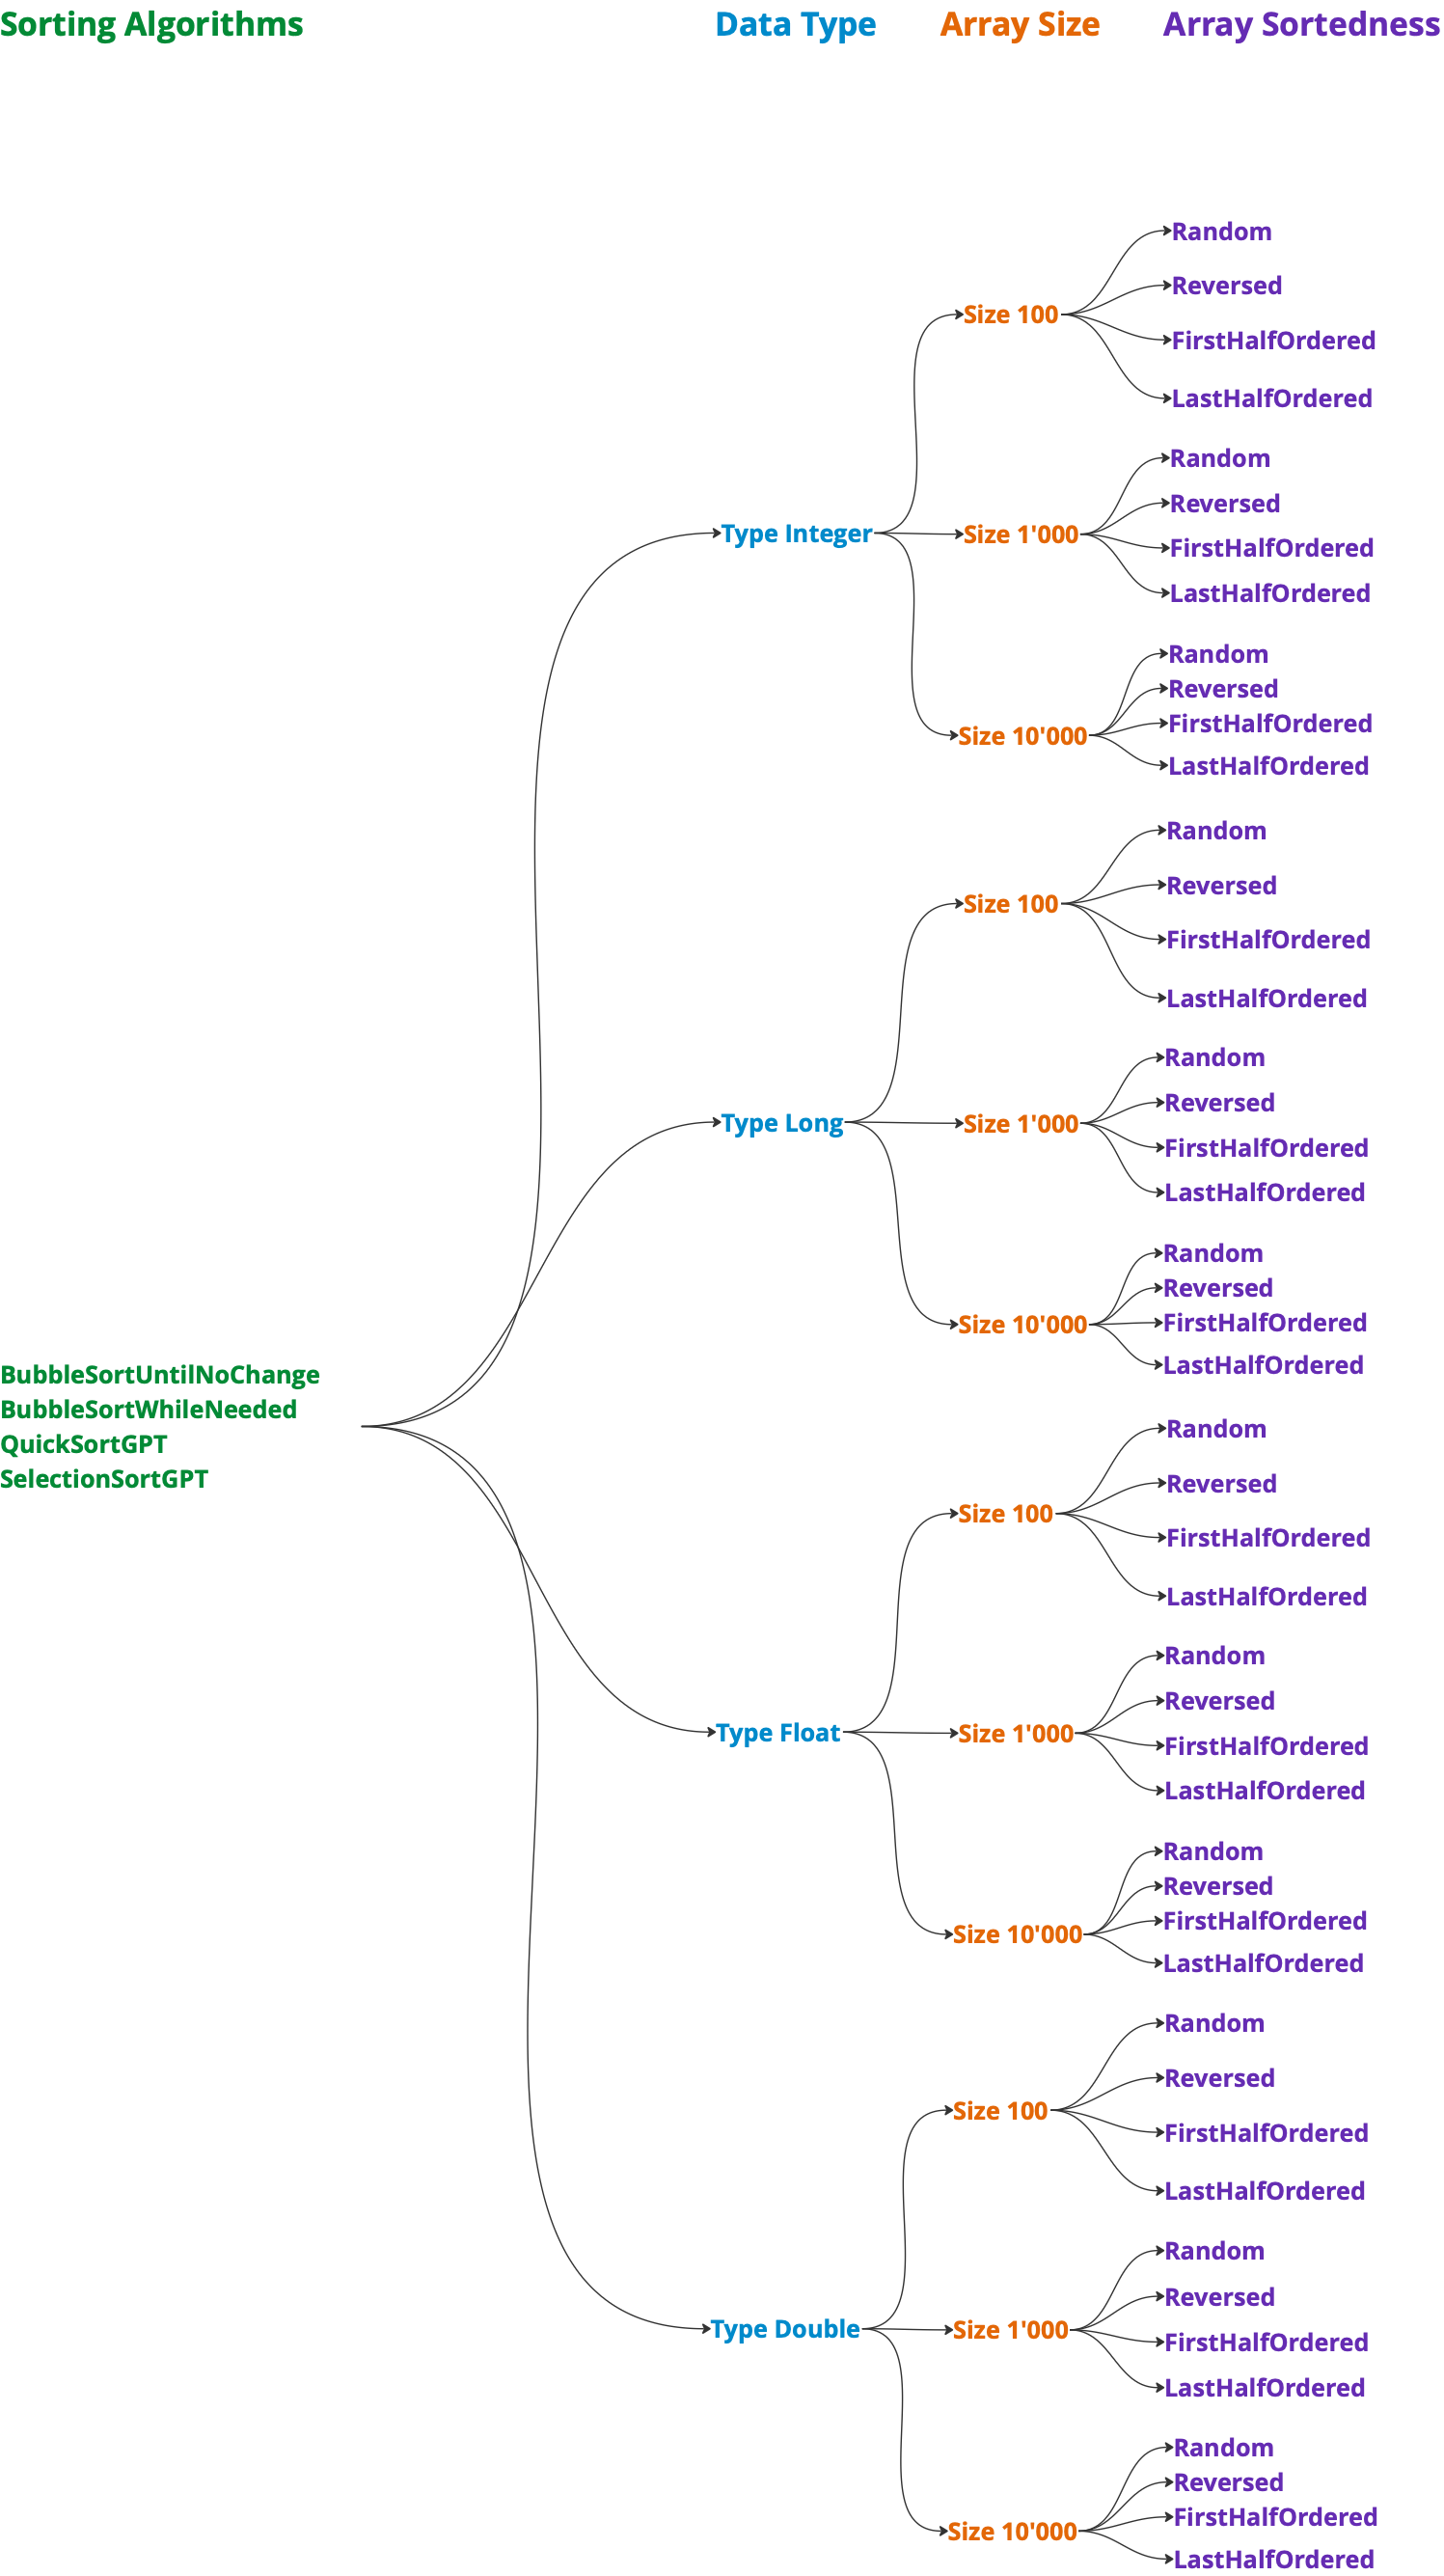
\includegraphics[width=0.8\textwidth]{./fig/factors.png}
            \caption{Factors in the experiment}
            \label{fig:factors}
        \end{figure}

    \end{itemize}

    \subsection{Apparatus and Materials}

    The experiment was conducted on a MacBook Air with an M1 chip, 8GB of RAM, running macOS Sequoia 15.1. The programming language used was OpenJDK 21.0.4, with VSCode version 1.92.1 as the integrated development environment (IDE). To ensure consistency and minimize interference, no other user processes were running in the background during the experiment.

    \subsection{Procedure}

    This is a high-level overview of the steps taken to conduct the experiment in terms of what the code does. \\

    \begin{enumerate}
        \item \textbf{Initialize Sorting Algorithms}:
        \begin{itemize}
            \item Define an array of sorting algorithms to test, each implementing a \texttt{sort} method (e.g., \texttt{BubbleSortUntilNoChange}, \texttt{BubbleSortWhileNeeded}, \texttt{QuickSortGPT}, \texttt{SelectionSortGPT}).
        \end{itemize}
    
        \item \textbf{Define Datasets}:
        \begin{itemize}
            \item Create datasets of varying sizes (100, 1,000, and 10,000) and data types (Integer, Long, Float, and Double).
            \item For each data type, initialize arrays for the specified sizes.
        \end{itemize}
    
        \item \textbf{Generate Dataset Configurations}:
        \begin{itemize}
            \item For each dataset, generate four initial configurations of data:
            \begin{itemize}
                \item \textbf{Random}: Populate the array with randomly generated values.
                \item \textbf{Reversed}: Populate the array with values in descending order.
                \item \textbf{First-half-sorted}: Sort the first half of the array, with the remaining elements randomized.
                \item \textbf{Last-half-sorted}: Sort the last half of the array, with the initial elements randomized.
            \end{itemize}
        \end{itemize}
    
        \item \textbf{Warm-Up Phase}:
        \begin{itemize}
            \item For each sorting algorithm, each dataset, and each sortedness level, perform an initial set of 25 sorting operations. These warm-up runs are discarded from the final results to allow the system and algorithm to stabilize.
        \end{itemize}
    
        \item \textbf{Measure Execution Time}:
        \begin{itemize}
            \item For each sorting algorithm, dataset size, data type, and sortedness level, perform 100 timed sorting operations:
            \begin{itemize}
                \item Use \texttt{System.nanoTime()} to measure the execution time for each sort.
                \item Record the time taken in nanoseconds for each sort in a CSV file.
            \end{itemize}
        \end{itemize}
    
        \item \textbf{Store Results}:
        \begin{itemize}
            \item Record the algorithm name, data type, data size, sortedness level, and time taken for each run in the CSV file to allow for subsequent analysis.
        \end{itemize}
    
        \item \textbf{Analyze Data}:
        \begin{itemize}
            \item Process the CSV file using python3.12.4 in a Jupyter Notebook to create graphs and tables, analyzing the relationship between independent variables (sorting algorithm, data size, data type, and sortedness level) and the dependent variable (execution time).
        \end{itemize}
    \end{enumerate}


\section{Results}

    \subsection{Visual Overview}


    \begin{figure}[htbp]
        \centering
        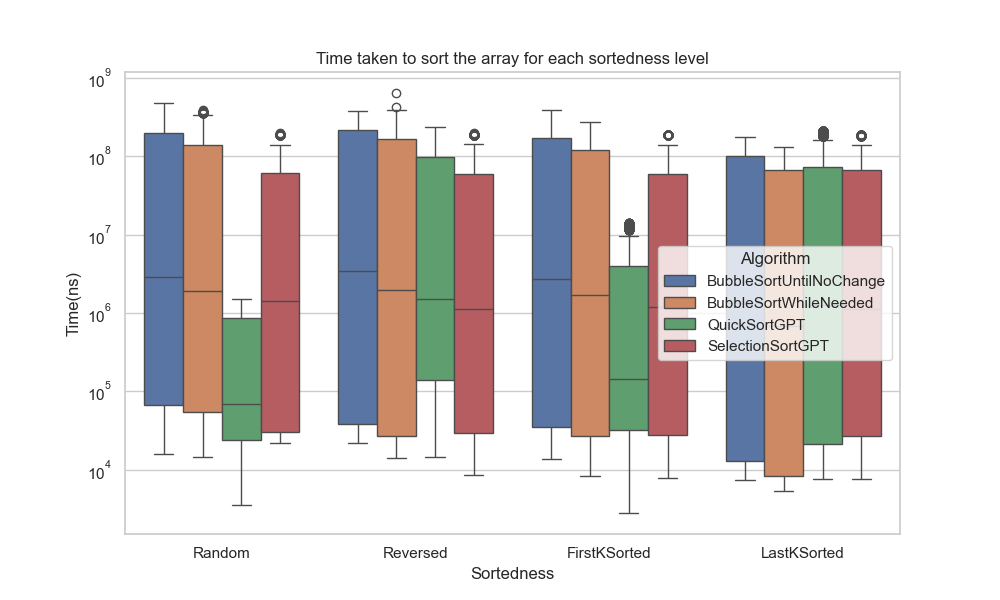
\includegraphics[width=0.8\textwidth]{./fig/hip1.png}
        \caption{Sortedness of input vs time in logarithmic scale}
        \label{fig:hip1}
    \end{figure}

    In Figure \ref{fig:hip1}, we show the relationship between the level of sortedness of the input data and the running time of the sorting algorithm. The x-axis represents the level of sortedness, while the y-axis (in logarithmic scale)represents the time in nanoseconds. The graph shows that the running time increases as the level of sortedness decreases. The relationship is more evident with the y-axis in linear scale, as shown in Figure \ref{fig:hip1_linear}.\\
    \hfill

    \begin{figure}[htbp]
        \centering
        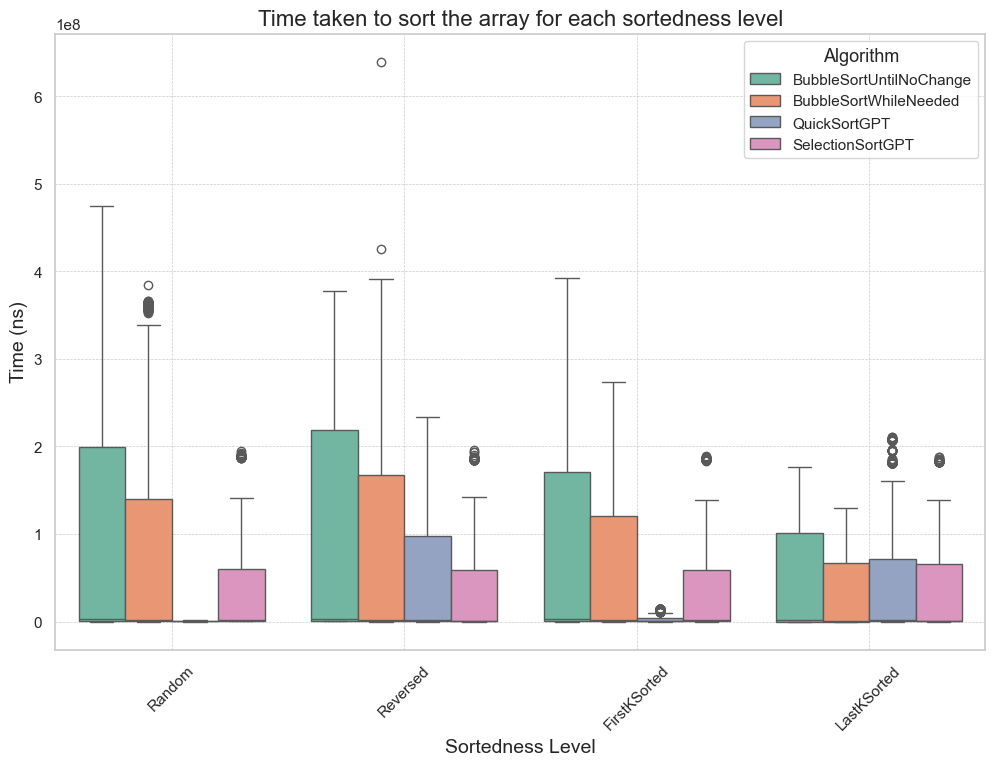
\includegraphics[width=0.8\textwidth]{./fig/hip1-nonLog.png}
        \caption{Sortedness of input vs time in linear scale}
        \label{fig:hip1_linear}
    \end{figure}

    In Figure \ref{fig:hip2}, we show the relationship between the size of the dataset and the running time of the sorting algorithm. The x-axis represents the size of the dataset, while the y-axis (in logarithmic scale) represents the time in nanoseconds. The graph shows that the running time increases as the size of the dataset increases. The relationship is more evident in the logarithmic scale.\\
\hfill



\begin{figure}[htbp]
    \centering
    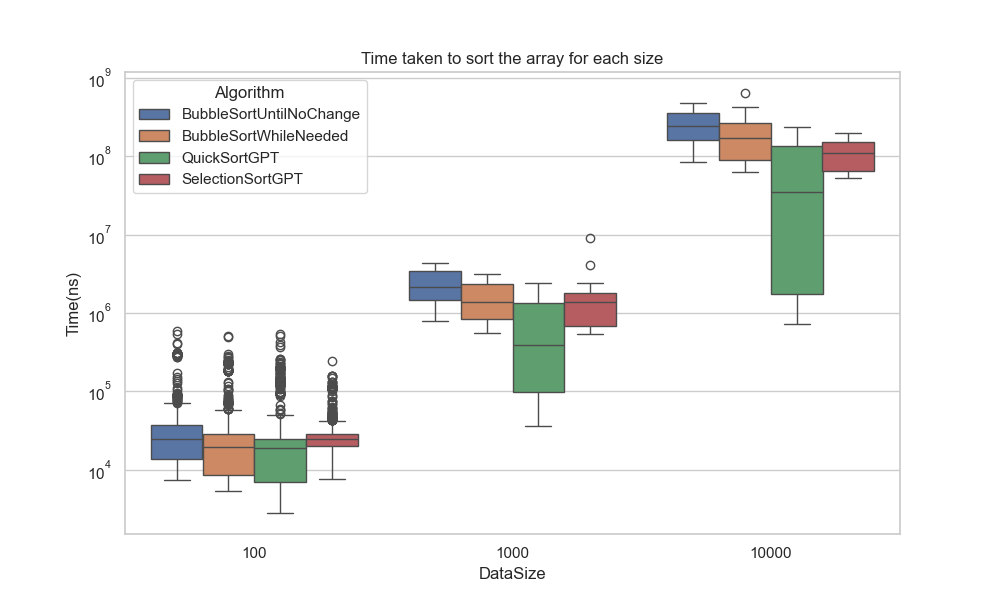
\includegraphics[width=0.8\textwidth]{./fig/hip2.png}
    \caption{Size of dataset vs time in logarithmic scale}
    \label{fig:hip2}
\end{figure}


    In Figure \ref{fig:hip3}, we show the relationship between the data type of the elements in the dataset and the running time of the sorting algorithm. The x-axis represents the data type, while the y-axis (in logarithmic scale) represents the time in nanoseconds. The graph shows that the running time varies across different data types, with Double (8B) having the highest running time. The relationship is more evident in the logarithmic scale.\\
\hfill
        \begin{figure}[htbp]
            \centering
            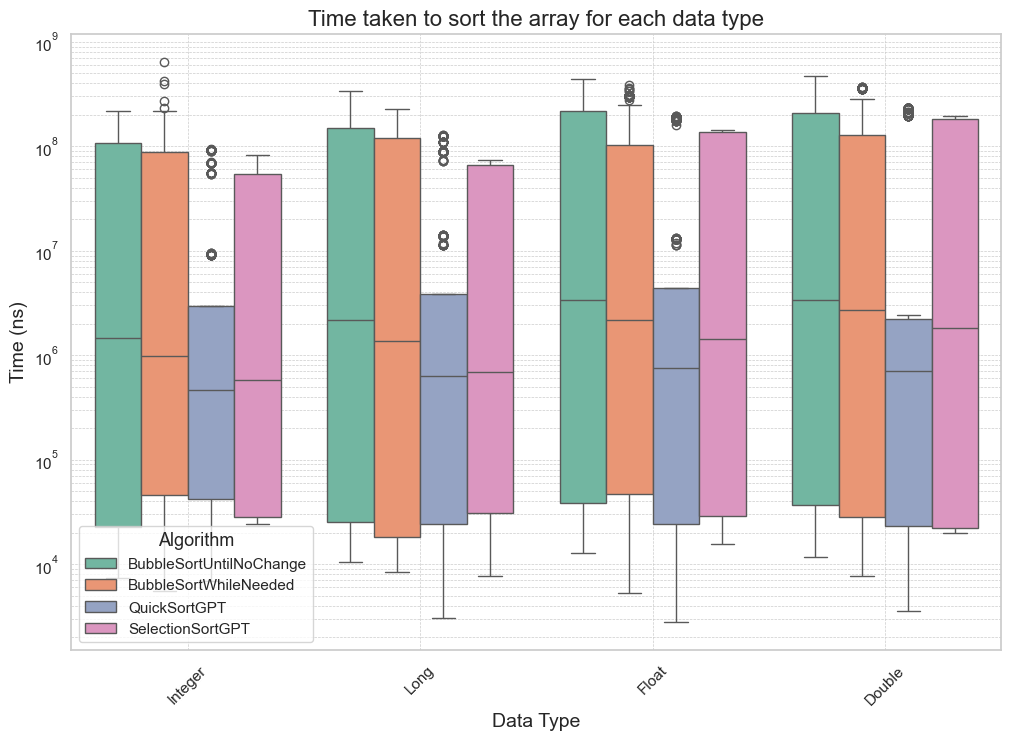
\includegraphics[width=0.8\textwidth]{./fig/hip3.png}
            \caption{Data type vs time in logarithmic scale}
            \label{fig:hip3}
        \end{figure}


    \subsection{Descriptive Statistics}

    The following tables provide a summary of the running times for each sorting algorithm, data type, and sortedness level. The tables include the minimum, 1st quartile, median, 3rd quartile, and maximum values for the running times in nanoseconds. The data is presented separately for each combination of sorting algorithm, sortedness level, and data type.\\

    \begin{center}
        \footnotesize
        \begin{longtable}{|l|l|l|r|r|r|r|r|}
            \hline
            \textbf{Algorithm} & \textbf{Sort} & \textbf{Type} & \textbf{min} & \textbf{1st Quartile} & \textbf{Median} & \textbf{3rd Quartile} & \textbf{max} \\
            \hline
            \endfirsthead
            \hline
            \textbf{Algorithm} & \textbf{Sort} & \textbf{Type} & \textbf{min} & \textbf{1st Quartile} & \textbf{Median} & \textbf{3rd Quartile} & \textbf{max} \\
            \hline
            \endhead
            \hline
            \endfoot
            BSUNC & FirstKSorted & Double & 34791.0 & 34875.0 & 3312062.0 & 343318844.0 & 351527666.0 \\
            BSUNC & FirstKSorted & Float & 30750.0 & 31072.75 & 3155375.0 & 350424322.75 & 392856209.0 \\
            BSUNC & FirstKSorted & Integer & 13583.0 & 14729.25 & 1343187.5 & 148487458.0 & 151545833.0 \\
            BSUNC & FirstKSorted & Long & 20541.0 & 20989.75 & 2004687.5 & 234806093.75 & 335577375.0 \\
            BSUNC & LastKSorted & Double & 11666.0 & 11750.0 & 1480958.0 & 160909833.25 & 165408292.0 \\
            BSUNC & LastKSorted & Float & 12708.0 & 12958.0 & 1457250.0 & 167002396.0 & 176130916.0 \\
            BSUNC & LastKSorted & Integer & 7333.0 & 7875.0 & 867541.5 & 91748813.0 & 97350042.0 \\
            BSUNC & LastKSorted & Long & 10458.0 & 11062.25 & 1136354.5 & 122797698.0 & 125335375.0 \\
            BSUNC & Random & Double & 32916.0 & 33042.0 & 3682646.0 & 424603208.0 & 474684667.0 \\
            BSUNC & Random & Float & 30791.0 & 87791.75 & 3400917.0 & 422298510.25 & 439274584.0 \\
            BSUNC & Random & Integer & 15666.0 & 133125.0 & 1492396.0 & 160357624.75 & 173614375.0 \\
            BSUNC & Random & Long & 20583.0 & 66531.5 & 2178979.0 & 276661135.75 & 310634458.0 \\
            BSUNC & Reversed & Double & 37000.0 & 37614.75 & 3387854.5 & 369365749.5 & 377215667.0 \\
            BSUNC & Reversed & Float & 35334.0 & 38375.0 & 3646688.0 & 368913708.25 & 375371000.0 \\
            BSUNC & Reversed & Integer & 21750.0 & 22584.0 & 1950646.0 & 205561052.25 & 215514250.0 \\
            BSUNC & Reversed & Long & 23916.0 & 25333.0 & 2318750.0 & 257731780.75 & 262898583.0 \\
            BSWN & FirstKSorted & Double & 26542.0 & 27770.5 & 2494000.0 & 269238020.75 & 273290750.0 \\
            BSWN & FirstKSorted & Float & 19291.0 & 19417.0 & 1994313.0 & 220615062.5 & 226031458.0 \\
            BSWN & FirstKSorted & Integer & 8208.0 & 8322.75 & 857646.0 & 94190728.75 & 109389625.0 \\
            BSWN & FirstKSorted & Long & 13375.0 & 14062.25 & 1201000.5 & 164325427.25 & 182960625.0 \\
            BSWN & LastKSorted & Double & 7750.0 & 8084.0 & 690875.0 & 79905770.75 & 82992583.0 \\
            BSWN & LastKSorted & Float & 5333.0 & 5417.0 & 573625.0 & 64216843.75 & 69149458.0 \\
            BSWN & LastKSorted & Integer & 5500.0 & 5625.0 & 590083.5 & 66779885.5 & 129658834.0 \\
            BSWN & LastKSorted & Long & 8334.0 & 8708.75 & 739145.5 & 81190062.25 & 111125875.0 \\
            BSWN & Random & Double & 28375.0 & 28583.0 & 3001229.5 & 359720093.5 & 366413042.0 \\
            BSWN & Random & Float & 46625.0 & 50239.5 & 2202333.0 & 300086094.0 & 384812458.0 \\
            BSWN & Random & Integer & 45042.0 & 47468.75 & 1002146.0 & 107917281.5 & 122899292.0 \\
            BSWN & Random & Long & 14458.0 & 59781.0 & 1402188.0 & 194750969.0 & 226067959.0 \\
            BSWN & Reversed & Double & 27083.0 & 27250.0 & 2690937.5 & 280814093.5 & 285547250.0 \\
            BSWN & Reversed & Float & 21625.0 & 24500.0 & 2434833.5 & 241278593.75 & 277258500.0 \\
            BSWN & Reversed & Integer & 13958.0 & 54562.0 & 1216875.0 & 153523864.75 & 639605292.0 \\
            BSWN & Reversed & Long & 17833.0 & 18042.0 & 1503917.0 & 167367146.25 & 171405667.0 \\
            QSGPT & FirstKSorted & Double & 3791.0 & 3834.0 & 147187.5 & 1903906.0 & 2212208.0 \\
            QSGPT & FirstKSorted & Float & 2792.0 & 3042.0 & 139333.0 & 12834749.75 & 13212750.0 \\
            QSGPT & FirstKSorted & Integer & 32333.0 & 48875.0 & 102208.5 & 9286667.25 & 9579167.0 \\
            QSGPT & FirstKSorted & Long & 3083.0 & 3167.0 & 151167.0 & 13716134.75 & 14160542.0 \\
            QSGPT & LastKSorted & Double & 21166.0 & 22000.0 & 1955250.5 & 207200749.75 & 211028916.0 \\
            QSGPT & LastKSorted & Float & 17042.0 & 17209.0 & 1840125.0 & 181340145.5 & 185499167.0 \\
            QSGPT & LastKSorted & Integer & 7500.0 & 93739.5 & 561541.5 & 68887509.75 & 71272667.0 \\
            QSGPT & LastKSorted & Long & 10250.0 & 10292.0 & 739646.0 & 88561885.0 & 90974583.0 \\
            QSGPT & Random & Double & 3583.0 & 3875.0 & 81479.5 & 1250177.25 & 1462875.0 \\
            QSGPT & Random & Float & 23792.0 & 24280.75 & 69708.0 & 1170760.25 & 1494041.0 \\
            QSGPT & Random & Integer & 6875.0 & 7655.75 & 37562.5 & 740969.0 & 839833.0 \\
            QSGPT & Random & Long & 23291.0 & 24041.75 & 53792.0 & 887865.0 & 1327291.0 \\
            QSGPT & Reversed & Double & 23375.0 & 23500.0 & 2221333.5 & 229394791.5 & 234112417.0 \\
            QSGPT & Reversed & Float & 18250.0 & 136677.75 & 1893042.0 & 188588510.75 & 195573416.0 \\
            QSGPT & Reversed & Integer & 41584.0 & 195208.0 & 765833.5 & 91154051.75 & 93264417.0 \\
            QSGPT & Reversed & Long & 14459.0 & 141229.0 & 1109583.0 & 125214010.25 & 127176375.0 \\
            SSGPT & FirstKSorted & Double & 21875.0 & 22583.0 & 1841437.5 & 184498437.5 & 188602875.0 \\
            SSGPT & FirstKSorted & Float & 17291.0 & 29989.5 & 1423271.0 & 136545218.75 & 138658833.0 \\
            SSGPT & FirstKSorted & Integer & 27541.0 & 28334.0 & 580250.0 & 54831750.0 & 56596041.0 \\
            SSGPT & FirstKSorted & Long & 7833.0 & 7989.75 & 688000.5 & 65361333.5 & 66988292.0 \\
            SSGPT & LastKSorted & Double & 20208.0 & 21030.75 & 1805854.5 & 182897791.0 & 188457666.0 \\
            SSGPT & LastKSorted & Float & 15583.0 & 15875.0 & 1388062.5 & 136043916.75 & 138951667.0 \\
            SSGPT & LastKSorted & Integer & 26667.0 & 28198.5 & 582562.0 & 55050457.75 & 82011875.0 \\
            SSGPT & LastKSorted & Long & 7666.0 & 8250.0 & 688687.5 & 65729291.25 & 68346333.0 \\
            SSGPT & Random & Double & 21791.0 & 21917.0 & 1861292.0 & 187903781.25 & 195235792.0 \\
            SSGPT & Random & Float & 28375.0 & 28697.75 & 1420229.0 & 136688541.75 & 140796417.0 \\
            SSGPT & Random & Integer & 26583.0 & 27239.75 & 582875.0 & 55168385.75 & 58463000.0 \\
            SSGPT & Random & Long & 30166.0 & 109656.5 & 690541.5 & 65995281.25 & 68053875.0 \\
            SSGPT & Reversed & Double & 19708.0 & 19792.0 & 1827187.5 & 184536437.75 & 195752416.0 \\
            SSGPT & Reversed & Float & 26375.0 & 43083.0 & 1391958.5 & 137661250.25 & 142159416.0 \\
            SSGPT & Reversed & Integer & 24459.0 & 25375.0 & 540395.5 & 53358979.25 & 55007000.0 \\
            SSGPT & Reversed & Long & 8500.0 & 30989.75 & 735229.0 & 72350291.0 & 74371750.0 \\
            \hline
        \end{longtable}
    \end{center}



\section{Discussion}

    \subsection{Compare Hypotheses with Results}
    
    Provide a brief restatement of the main results from the previous section, and if (or if not) these support your research hypothesis.\\

    If there is a discrepancy between your hypothesis and the results of your experiment, speculate about why you were unable to find evidence to support your hypothesis. 


    \subsection{Limitations and Threats to Validity}

    // TODO
    Acknowledge any faults or limitations your study has, and how seriously these affect your results. How could these be remedied in future work?


    \subsection{Conclusions}

    // TODO
    
    End with the main conclusions that can be drawn from your study.

\section{Appendix}

    \subsection{Reproduction Package}
    All of the code used to conduct the experiment, as well as the Jupyter Notebook used for data analysis and the Latex files for the report, can be found at the following GitHub repository: \url{https://github.com/costanza1234/USI-Exp-Eval-24}.

\end{document}